% vim: spell spelllang=es:
\documentclass[12pt, oneside]{article}
\usepackage[a4paper, left=2.5cm, right=2.5cm, top=2.5cm, bottom=2.5cm]{geometry}

\usepackage[utf8]{inputenc} % Use unicode
\usepackage[T1]{fontenc}
\usepackage[spanish,es-tabla]{babel} % Names in spanish


\usepackage{xcolor}
\usepackage{siunitx}

%% Bibliography:
%\usepackage{comment}
%\usepackage[
    %backend=biber,
    %style=numeric,
%]{biblatex}
%\DeclareNameAlias{default}{last-first}

%\usepackage{csquotes}       % For bibliography quotations
%\DeclareQuoteAlias{spanish}{catalan}

%\addbibresource{biblio.bib}
%% see:
%% https://www.sharelatex.com/learn/Bibliography_management_in_LaTeX#The_bibliography_file

%\usepackage{datetime} % Customize date
%% \monthyeardate\today gives the date without the day
%\newdateformat{monthyeardate}{%
    %\monthname[\THEMONTH], \THEYEAR}

% For cross references
\PassOptionsToPackage{hyphens}{url}\usepackage[colorlinks = true]{hyperref}
\usepackage[catalan]{varioref}
%\usepackage{cleveref}
%hyperref configuration so that it doesn't contrast so much colorlinks,
\hypersetup{
   linkcolor={black},
   citecolor={black},
   %linkcolor={red!50!black},
   %citecolor={blue!50!black},
   urlcolor={blue!80!black}
}

\usepackage{mathtools}  % amsmath + more
\usepackage{amsthm}     % Theorem enviroment
\usepackage{amssymb}    % More symbols
\usepackage{amstext}    % Text inside mathenv

\usepackage{relsize}    % Bigger math with mathlarger{___}
\usepackage{nicefrac}   % nice fractions in one line

\usepackage[export]{adjustbox}  % Adjust table size
\usepackage{float}              % Force tables and images position (H and H!)
\usepackage{wrapfig}            % Wrap images like in HTML

\usepackage{tabularx, colortbl, booktabs}    % Better tables
\usepackage{longtable}                      % Multiple page table

% Split cell in lines and more formating options inside table
\usepackage{array, multirow, multicol, makecell}

%\usepackage{subcaption}                     % Subfigures
%\usepackage[framemethod=tikz]{mdframed}     % Custom frames

%\usepackage[bottom]{footmisc} % Footnotes at bottom of page

%\usepackage[alsoload=hep]{siunitx}          % SI units and uncertainties
%\sisetup{locale = FR}                       % Commas and so on for spanish
%\sisetup{separate-uncertainty=true}
%\sisetup{
  %per-mode=fraction,
  %fraction-function=\nicefrac
%}

%\usepackage{tikz}
%%\usetikzlibrary{arrows}
%%\usetikzlibrary{scopes}
%\usetikzlibrary{babel}

%\usepackage{listings}       % For code blocks

%% Custom code highlight
%\definecolor{codegreen}{rgb}{0,0.6,0}
%\definecolor{codegray}{rgb}{0.5,0.5,0.5}
%\definecolor{codepurple}{rgb}{0.58,0,0.82}
%\definecolor{backcolour}{rgb}{0.95,0.95,0.92}
%\definecolor{lightblue}{RGB}{135,206,250}

%\lstdefinestyle{mystyle}{ backgroundcolor=\color{backcolour},
    %commentstyle=\color{codegreen}, keywordstyle=\color{blue},
    %numberstyle=\tiny\color{codegray}, stringstyle=\color{red},
    %identifierstyle=\color{black}, basicstyle=\footnotesize,
    %%breakatwhitespace=false,
    %breaklines=true,
    %%captionpos=b,                    keepspaces=true,
    %numbers=left,                    numbersep=5pt,
    %showspaces=false,
    %%showstringspaces=false, showtabs=false,
    %tabsize=4
%}
%\lstset{style=mystyle}

\newcommand{\whitepage}{
    \clearpage\thispagestyle{empty}\addtocounter{page}{-1} \newpage \clearpage
}

% Add command before appendix session for page numbering: A-1
%\newcommand{\appendixpagenumbering}{
    %\break
    %\pagenumbering{arabic}
    %\renewcommand{\thepage}{\thesection-\arabic{page}}
%}

%% Custom Math operators (functions not in italic in math mode):
%\DeclareMathOperator{\arcsec}{arcsec}
%\DeclareMathOperator{\arccot}{arccot}
%\DeclareMathOperator{\arccsc}{arccsc}
%\DeclareMathOperator{\cis}{cis}


\usepackage[bottom]{footmisc}

\usepackage{amsmath}
\usepackage[justification=centering]{caption}

\title{%
IA: Trabajo de innovación
}

\author{%
    Aleix Boné\\
    Alex Herrero\\
    Moisés Balcells
}
\date{%
Mayo 2020
}

\begin{document} 


\thispagestyle{empty}
\clearpage
\setcounter{page}{-1}

\begin{titlepage}
{
    \centering
    \null
    \vfill
    {\Large Inteligencia Artificial\par}
    \vspace{2em}
    {\Huge \bfseries 
    Trabajo de innovación \\
    AIRx %\textsuperscript{TM}
    \par}
    \vspace{2em}
    {\large \scshape 
    Mayo 2020
    \par}
    \vfill
\begin{center}
    
\end{center}
    \vspace{3cm}

    \vfill
    {\raggedleft \large
Aleix Boné Ribó\\
Alex Herrero Pons\\
    Moisés Balcells
        \par}
}
\end{titlepage}

\pagebreak

\thispagestyle{empty}
\clearpage
\setcounter{page}{0}

\tableofcontents

\pagebreak

%\section{Trabajo de innovación}
%
%El tema sobre el que trabajaremos es el escaneo inteligente con deep learning aplicado a la resonancia magnética. 
%En este ámbito la inteligencia artificial se utiliza para hacer el escaneo de imágenes más preciso y rápido. 
%En concreto nos centraremos en el producto AIRx™ de general electric healthcare.


%     Descripción del producto o servicio
%     Descripción de las técnicas de IA que se han utilizado
%     Descripción de cómo han sido utilizadas las técnicas
%     Explicación de porqué es un producto/servicio innovador y la naturaleza de la innovación (innovación en la técnica/método de IA, uso innovador de técnicas ya existentes)
%     Impacto del producto en la empresa (beneficios, riesgos, posición en el mercado)
%     Impacto del producto en el usuario o en la sociedad (beneficios y riesgos)
%      Bibliografía/Referencias utilizadas para la elaboración del documento


% solo se tiene k ir mirando en las fuentes k tenemos y ir metiendo

% btw quizás estaría bien poner en la portada el nombre de nuestro producto

% y el cuestionario del trabajo en equipo del trabajo de innovación lo entregasteis? porque yo no :o
% no
% no creo que importe mucho
% ya esta la biblio como tocaria
% si encontrais otra pagina web o algo apunta el link abajo i la meto. okkay perff


\section{Introducción}
Actualmente, en el campo de la medicina hay diversas técnicas para observar alteraciones en los tejidos y detectar cáncer y otras patologías. Una de las técnicas más conocidas y utilizadas es el análisis de imágenes creadas por resonancia magnética (MRI). 

La MRI es una técnica no invasiva que hace uso del fenómeno de la resonancia magnética nuclear para extraer información sobre la estructura y composición del cuerpo a analizar.

Esta información es procesada por ordenadores y transformada en imágenes.

%La resonancia magnética ( MRI ) es una técnica de imagen médica utilizada en radiología para formar imágenes de la anatomía y los procesos fisiológicos del cuerpo. Los escáneres de resonancia magnética utilizan campos magnéticos fuertes , gradientes de campo magnético y ondas de radio para generar imágenes de los órganos del cuerpo.La IRM (Figura 1) es una técnica de imagen en 3D que permite a los médicos visualizar estructuras en el cuerpo de manera no invasiva y sin radiación ionizante. La resonancia magnética es una modalidad de imagen muy utilizada y potente debido a su contraste superior entre los tejidos "blandos", por ejemplo, materia gris, materia blanca y LCR, así como su capacidad única no solo de visualizar estructuras anatómicas, sino también de representar fisiología y función, p. Ej. flujo sanguíneo, perfusión y difusión.

% Esta información es procesada por ordenadores y transformada en imágenes del interior de lo que se ha analizado.

% También es utilizada industrialmente para analizar la estructura de materiales tanto orgánicos como inorgánicos. 

\section{Descripción del producto}
El producto escogido es AIR este tiene el objetivo de realizar un escaneo de resonancia magnética (MRI) mediante inteligencia artificial y este incorpora un módulo basado en el aprendizaje profundo que se llama AIRx.
\cite{noauthor_magnetic_nodate} 
    \subsection{MRI} % IRM en castellano
    % aqui que ponemos?? porque yo iba a hablar de la MRI en la intro
    %no sé
    % yo pondria en mas detalle como se hace un MRI
    % para poder decir en que ayuda el producto.
    % es decir, para hacer un MRI el operador tiene que hacer esto y esto manualemtne y 
    % es dificl i se tarda much o y si se hace mal que pasa y todo ese rollo.
    En el examen de MRI, el operador de exploración primero adquiere un conjunto de imágenes de "localizador" de baja resolución (figura~\ref{fig:resonancia}) a partir de las cuales se puede identificar la ubicación y orientación aproximadas de los puntos de referencia deseados. Estas referencias anatómicas se utilizan para planificar manualmente las ubicaciones exactas, la orientación y la cobertura requerida para las imágenes que se utilizarán para los escaneos de alta resolución que se utilizan para el diagnóstico. Este procedimiento es complicado ya que la orientación, la ubicación y la cobertura deben ser correctas en las tres dimensiones
     espaciales.
     
     \begin{figure}[H]
        \centering
        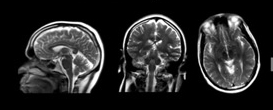
\includegraphics[width=0.9\textwidth]{resonancia.png}
        \caption{Imagen MRI}%
        \label{fig:resonancia}
     \end{figure}
    
    La calidad y la consistencia del posicionamiento y la orientación de los cortes depende en gran medida de la habilidad y experiencia del operador de escaneo. Este proceso puede llevar mucho tiempo y ser difícil, especialmente para las anatomías complejas. Como resultado, puede haber inconsistencias de un operador de escaneo a otro. Esta falta de consistencia puede hacer que el trabajo del radiólogo al interpretar estas imágenes sea más difícil, especialmente cuando un paciente está siendo escaneado como un seguimiento de un examen de resonancia magnética anterior y están tratando de identificar cambios sutiles en la anatomía o la progresión de la enfermedad con el tiempo. En el peor de los casos, no se obtienen las imágenes correctas y el paciente debe regresar para otro procedimiento.
    \subsection{Antecedentes}
    %..
    \subsection{AIRx}
    El módulo AIRx incorpora tecnología CNN, a este módulo el tiempo que le toma al operador de exploración determinar las ubicaciones y orientaciones para los planos de exploración deseados para una resonancia magnética cerebral puede reducirse entorno al 40-60 por ciento. Y además gracias a este módulo se puede ver una reducción en los errores y una precisión mejorada. Esto se puede traducir como  resultados de exámenes generales más cortos,con una posibilidad reducida de devolución de llamadas del paciente y una mejor calidad de diagnóstico del examen.
\section{Técnicas de IA}

    La principal técnica de IA utilizada son redes neuronales convolucionales.

    \subsection{Convolutional Neural Networks (CNN)}
    
    Las redes neuronales convolucionales son un caso especifico de redes neuronales de deep learning
    en las que la entrada son imágenes. Son redes de clasificación feed-forward (no son recurrentes)
    
     \begin{figure}[H]
        \centering
        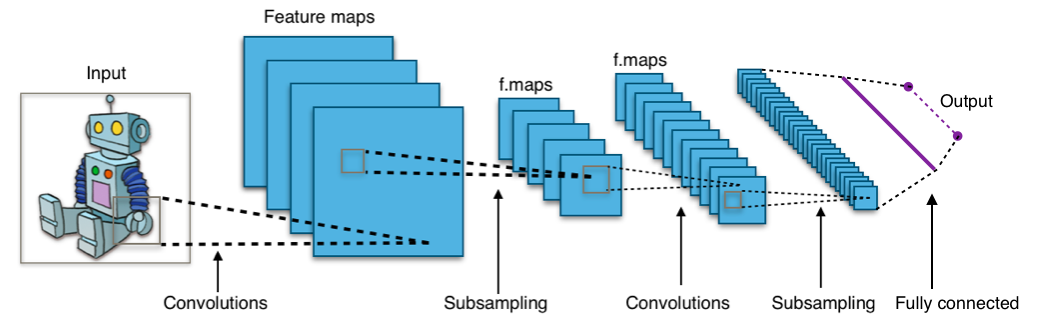
\includegraphics[width=0.9\textwidth]{cnn}
        \caption{CNN}%
        \label{fig:cnn}
     \end{figure}
    
    % https://torres.ai/deep-learning-inteligencia-artificial-keras/#5_REDES_NEURONALES_CONVOLUCIONALES
    
    \subsection{U-net}
    
    U-net es un tipo de CNN para la segmentación de imágenes, es decir dividir la imagen inicial en
    segmentos. La idea principal es aplicar una CNN con capas de pooling (reducen el tamaño de la entrada
    augmentando la información de las características), una vez se tiene la información se aplica otra
    CNN con capas de up-conv que usan la información de las capas de pooling para aumentar el tamaño
    de la salida hasta generar un mapa de segmentación de la imagen en las dimensiones originales de la
    entrada. En la figura~\ref{fig:unet} se ve un ejemplo de U-net (se puede apreciar también la forma de
    U del diagrama que le da el nombre a la red).
    
     \begin{figure}[H]
        \centering
        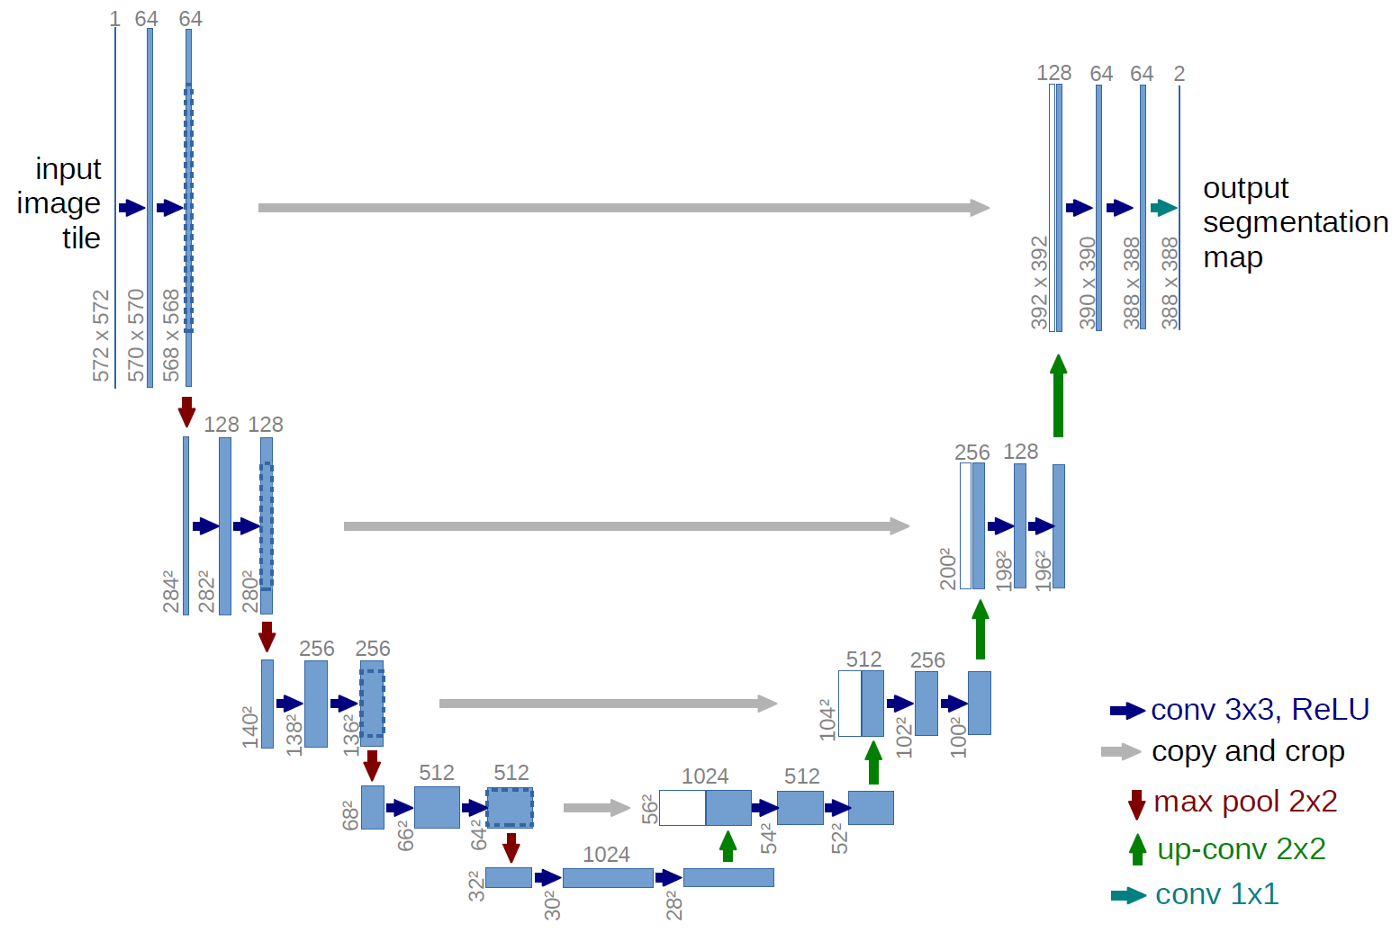
\includegraphics[width=0.9\textwidth]{unet}
        \caption{U-net}%
        \label{fig:unet}
     \end{figure}
     
\section{Uso de las técnicas de IA}
\cite{noauthor_intelligent_nodate}
\cite{noauthor_magnetic_nodate} 
\cite{noauthor_new_nodate}

El proceso se divide en 3 etapas \cite{noauthor_ge_nodate-1}:
\emph{LocalizerIQ-Net}, \emph{Coverage-Net} y \emph{Orientation-Net}, cada una de ellas usa varias 
CNNs distintas.

     \begin{figure}[H]
        \centering
        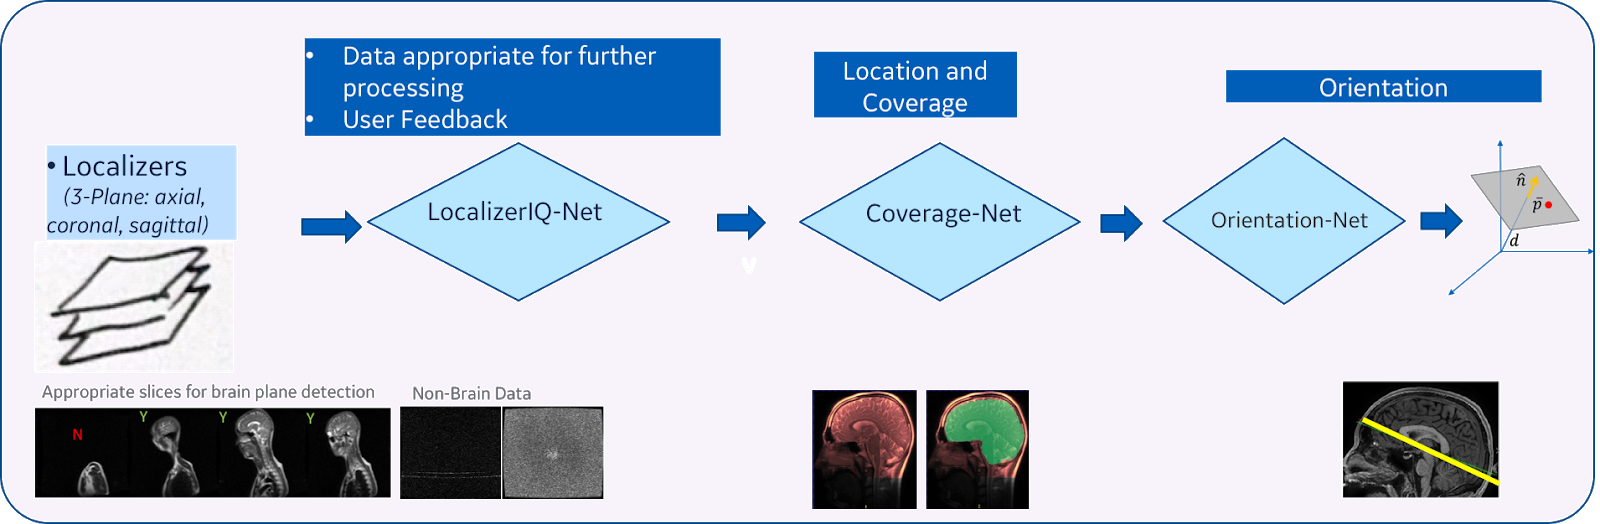
\includegraphics[width=0.9\textwidth]{steps}
        \caption{Etapas}%
        \label{fig:steps}
     \end{figure}

    \subsection{LocalizerIQ-Net}
    
    Esta etapa decide para cada una de las imágenes de localización iniciales si es útil para
    identificar el plano de la anatomía deseada. Esto sirve para identificar si las imágenes iniciales
    son buenas y útiles para las siguientes fases o si el operador debe realizar mas escáneres.
    
    En esta etapa se usa una red neuronal convolutional de clasificación de 5 capas con 
    
    %Image quality inspection: In the first step, we check if the given localizer image is suitable to identify the plane for the desired anatomy. This is achieved by using a fiver layer, dyadic reduction regular CNN classification network model (that we call “LocalizerIQ-Net”) to identify slices with relevant brain-anatomy, slices with artifacts and irrelevant slices. If the localizer image is not suitable for ISP, relevant feedback is provided to the scan operator. We used the built-in TensorFlow functions for image manipulation to achieve data augmentation during the training of LocalizerIQ-Net.
    
    \subsection{Coverage-Net}
    %Identification of anatomy coverage: Next, we locate the spatial-extent of the desired anatomy (brain) in the localizer images by incorporating a shape-based semantic image segmentation U-Net DL model (called “Coverage-Net”). This helps the next processing steps to be robust to changes in imaging parameter settings across hospitals and clinics as well as changes in shapes and sizes of the patient’s anatomy.
    \subsection{Orientation-Net}
    
    % Identification of precise plane orientation and location: For each desired anatomic structure (example, optic nerve), we find the scan-plane that is best suited to image that structure using one or more image segmentation 3D U-Net models (called “Orientation-Net”). Orientation-Net directly segments the desired-planes on localizer images, which is then used to compute the orientation and location.
    
\section{Explicación de la innovación}
\cite{noauthor_intelligent_nodate}
\cite{noauthor_magnetic_nodate} 

La naturaleza de la innovación reside en el uso de IA en una etapa del MRI donde no se había usado antes.
Como hemos mencionado, el uso de CNN se ha usado anteriormente en el ámbito de los MRI para examinar
los resultados obtenidos y ayudar en el diagnostico (detectar metástasis, etc.). Sin embargo
este producto introduce el uso de técnicas de MRI para facilitar la realización de los escaneres y
obtener los mejores slices posibles.

\section{Impacto del producto en la empresa}

\cite{noauthor_intelligent_nodate}
\cite{noauthor_new_nodate}

    \subsection{Beneficios}
    
    El principal beneficio es la mejora en la eficiencia y la calidad de las imágenes obtenidas en el
    MRI, que permiten un diagnostico mas rápido y fiable.
    
    \subsection{Riesgos}
    
    \subsection{Posición en el mercado}
    
\section{Impacto del producto en el usuario o en la sociedad}
\cite{noauthor_new_nodate}
\cite{noauthor_magnetic_nodate} 

    \subsection{Beneficios}
    \subsection{Riesgos}
    
    
\pagebreak

% TODO: quitar esto
6 \cite{noauthor_intelligent_nodate} %.
5 \cite{noauthor_how_nodate}
9 \cite{noauthor_magnetic_nodate}  %.
10 \cite{noauthor_new_nodate} %.
8 \cite{justo_exploring_nodate}
2 \cite{noauthor_deep-learning_nodate}
3 \cite{noauthor_ge_nodate}
7 \cite{noauthor_introducing_nodate}
1 \cite{bien_dont_2018}
4 \cite{noauthor_ge_nodate-1}

\sloppy
\printbibliography

\end{document}

%%%%%%%%%%%%%%%%%%%%%%%%%%%%%%%%%%%%%%%%%%%%%%%%%%%%%%%%%%%%%%%%%%%%%%%%%%%%%%%%
% END
%%%%%%%%%%%%%%%%%%%%%%%%%%%%%%%%%%%%%%%%%%%%%%%%%%%%%%%%%%%%%%%%%%%%%%%%%%%%%%%%

%%%%%%%%%%%%%%%%%%%%%%%%%%%%%%%%%%%%%%%%%%%%%%%%%%%%%%%%%%%%%%%%%%%%%%%%%%%%%%%%
% URLs bibliografia que faltan
%%%%%%%%%%%%%%%%%%%%%%%%%%%%%%%%%%%%%%%%%%%%%%%%%%%%%%%%%%%%%%%%%%%%%%%%%%%%%%%%

% meted aqui si encontrais algo util

%%%%%%%%%%%%%%%%%%%%%%%%%%%%%%%%%%%%%%%%%%%%%%%%%%%%%%%%%%%%%%%%%%%%%%%%%%%%%%%%
% Apartados bibliografia
%%%%%%%%%%%%%%%%%%%%%%%%%%%%%%%%%%%%%%%%%%%%%%%%%%%%%%%%%%%%%%%%%%%%%%%%%%%%%%%%

% https://blog.tensorflow.org/2019/03/intelligent-scanning-using-deep-learning.html?m=1   
% - Descripción del producto
% - técnicas de IA utilizadas
% - como se han utilizado las técnicas
% - impacto en la empresa
\cite{noauthor_intelligent_nodate}

% https://www.gehealthcare.com/article/magnetic-resonance-imaging-using-ai-a-new-deep-learning-tool   
% - Descripción del producto
% - técnicas de IA utilizadas
% - impacto en el usuario o la sociedad
\cite{noauthor_magnetic_nodate}

% https://www.gehealthcare.com/article/how-advanced-applications-and-ai-are-impacting-mri  
% - Técnicas de IA utilizadas
% - impacto en el usuario o la sociedad
\cite{noauthor_how_nodate}

% http://www.gesignapulse.com/signapulse/spring_2019/MobilePagedArticle.action?articleId=1488815&app=false#articleId1488815 
% - Técnicas de IA utilizadas
% - como se han utilizado las técnicas
% - impacto en el usuario o en la empresa)
\cite{noauthor_new_nodate}

% http://www.gesignapulse.com/signapulse/spring_2018/MobilePagedArticle.action?articleId=1396203&app=false#articleId1396203 
% - Descripción del producto
% - impacto del producto en el usuario o en la sociedad
% - impacto del producto en la empresa
\cite{justo_exploring_nodate}

% https://www.auntminnie.com/index.aspx?sec=rca&sub=ecr_2019&pag=dis&ItemID=124750  
% - técnicas IA utilizadas
% - impacto del producto en el usuario o en la sociedad
% - impacto del producto en la empresa
\cite{noauthor_deep-learning_nodate}

% https://www.dotmed.com/news/story/46576    
% - Descripción del producto
% - impacto del producto en el usuario o en la sociedad
% - impacto del producto en la empresa
\cite{noauthor_ge_nodate}

% http://www.gesignapulse.com/signapulse/autumn_2018/MobilePagedArticle.action?articleId=1444512&app=false#articleId1444512  
% - Descripción del producto
% -  técnicas de IA utilizadas
\cite{noauthor_introducing_nodate}

% https://medium.com/stanford-ai-for-healthcare/dont-just-scan-this-deep-learning-techniques-for-mri-52610e9b7a85   
% - Descripción del producto
% - técnicas de IA utilizadas
% - como se han utilizado las técnicas
\cite{bien_dont_2018}

% https://www.intel.com/content/www/us/en/artificial-intelligence/solutions/gehc-airx.html
\cite{noauthor_ge_nodate-1}

%%%%%%%%%%%%%%%%%%%%%%%%%%%%%%%%%%%%%%%%%%%%%%%%%%%%%%%%%%%%%%%%%%%%%%%%%%%%%%%%%%%%%%%%%%%%%%%%%%%
% equivalencias de url a cite en la bibliografía
%%%%%%%%%%%%%%%%%%%%%%%%%%%%%%%%%%%%%%%%%%%%%%%%%%%%%%%%%%%%%%%%%%%%%%%%%%%%%%%%%%%%%%%%%%%%%%%%%%%
 
% https://blog.tensorflow.org/2019/03/intelligent-scanning-using-deep-learning.html \cite{noauthor_intelligent_nodate}
%https://www.gehealthcare.com/article/how-advanced-applications-and-ai-are-impacting-mri \cite{noauthor_how_nodate}
%https://www.gehealthcare.com/article/magnetic-resonance-imaging-using-ai-a-new-deep-learning-tool \cite{noauthor_magnetic_nodate}
%http://www.gesignapulse.com/signapulse/spring_2019/MobilePagedArticle.action?articleId=1488815 \cite{noauthor_new_nodate}
%http://www.gesignapulse.com/signapulse/spring_2018/MobilePagedArticle.action?articleId=1396203 \cite{justo_exploring_nodate}
%https://www.auntminnie.com/index.aspx?sec=rca&sub=ecr_2019&pag=dis&ItemID=124750 \cite{noauthor_deep-learning_nodate}
%https://www.dotmed.com/news/story/46576 \cite{noauthor_ge_nodate}
%http://www.gesignapulse.com/signapulse/autumn_2018/MobilePagedArticle.action?articleId=1444512 \cite{noauthor_introducing_nodate}
%https://medium.com/stanford-ai-for-healthcare/dont-just-scan-this-deep-learning-techniques-for-mri-52610e9b7a85 \cite{bien_dont_2018}
%https://www.intel.com/content/www/us/en/artificial-intelligence/solutions/gehc-airx.html \cite{noauthor_ge_nodate-1}

%%%%%%%%%%%%%%%%%%%%%%%%%%%%%%%%%%%%%%%%%%%%%%%%%%%%%%%%%%%%%%%%%%%%%%%%%%%%%%%%%%%%%%%%%%%%%%%%%%%

